\documentclass[10pt,a4paper]{article}
\usepackage[UTF8]{ctex}
\usepackage{amsmath}
\usepackage{amsfonts}
\usepackage{amssymb}
\usepackage{float}
%\usepackage{clrscode}
\usepackage[]{algorithm2e}
\usepackage{listings}
\lstset{
  basicstyle=\small,
  numbers=left,
  keywordstyle=\color{blue},
  numberstyle={\tiny\color{lightgray}},
  stepnumber=1, %行号会逐行往上递增
  numbersep=5pt,
  commentstyle=\small\color{red},
  backgroundcolor=\color[rgb]{0.95,1.0,1.0},
  showspaces=false,
  showtabs=false,
  frame=shadowbox, framexleftmargin=5mm, rulesepcolor=\color{red!20!green!20!blue!20!},
% frame=single,
%  TABframe=single,
  tabsize=4,
  breaklines=tr,
  extendedchars=false %这一条命令可以解决代码跨页时,章节标题,页眉等汉字不显示的问题
}
\usepackage{graphicx}
% Set the margin of document.
\usepackage[top=10mm, bottom=12.5mm, left=12.5mm, right=12.5mm]{geometry}
\usepackage{longtable}
\usepackage{float}
\renewcommand\figurename{图}
\renewcommand\tablename{表}
\title{简单物理实验的模拟}
\author{袁略真\\3130103964\\生物信息学\\浙江大学}
\begin{document}
\maketitle
\section{两个简谐振动的合成}
\subsection{基本原理}
振动方向相同的两个简谐振动
$$x_1 = A_1cos(\omega_1 t+\phi_1)$$
$$x_2 = A_2cos(\omega_2 t+\phi_2)$$

它们的合振动为$$x=x_1+x_2$$
\subsection{程序流程}
\begin{algorithm}[H]
\KwIn{$A_1,A_2,\omega_1,\omega_2,\phi_1,\phi_2,file$}
\KwOut{a table of $x_1,x_2,x,t$ stored in $file$}
\For{$t \gets 0$ \KwTo N-1}{
	$x_1 \gets A_1cos(\omega_1 t+\phi_1)$\;
	$x_2 \gets A_2cos(\omega_2 t+\phi_2)$\;
	$x \gets x_1 + x_2$\;
	print $x_1,x_2,x,t$ to $file$
}
 \caption{两个简谐振动的合成}
\end{algorithm}

程序中每隔1个单位时间计算一次位移,为得到比较光滑的曲线,应使得周期$T>>1$.

由于$T = \frac{2\pi}{\omega}$,故要求$w_1 \leqslant 0.3,\ w_2 \leqslant 0.3$.其他参数影响不大.

\subsection{改进}
有如下一些场合可能影响精度,对此做出相应改进
\begin{enumerate}
\item 用户通常希望输入含有$\pi$的数值给$\phi_1,\phi_2$).改进方法是让用户输入$\pi$前的系数,乘积由程序计算.
\item C/C++ 中浮点数的存储方式导致在数学上一样大小的数,计算机存储的数有微小差异.常用的方法是设置一个很小的阈值,差小于阈值认为比较的两个数相等.我将阈值设为0.000001.%然而存在一些情况,差值超过阈值(例如: A1=A2=$10^{10},\omega_1=\omega_2=0.1,\psi_1=0,\psi_2=\pi$,浮点数精度的差异会因A放大).
\end{enumerate}
\subsection{模拟及结果}
\subsubsection{模拟的参数设置}

\begin{table}[H]
\begin{minipage}[b]{0.2\linewidth}\centering
\begin{tabular}{cc}
\hline
$A1: 1$ &$A2: 1$\\
$w1: 0.1$ &$w2: 0.1$\\
$phi1: 0$ &$phi2: 0$\\
\hline
\end{tabular}
\caption{模拟1参数}\label{tab:8}
\end{minipage}
\hspace{0.5cm}
\begin{minipage}[b]{0.2\linewidth}\centering
\begin{tabular}{cc}
\hline
$A1: 1$ &$A2: 1$\\
$w1: 0.1$ &$w2: 0.1$\\
$phi1: 0$ &$phi2: \pi$\\
\hline
\end{tabular}
\caption{模拟2参数}\label{tab:9}
\end{minipage}
\hspace{0.5cm}
\begin{minipage}[b]{0.2\linewidth}\centering
\begin{tabular}{cc}
\hline
$A1: 1$ &$A2: 1$\\
$w1: 0.1$ &$w2: 0.15$\\
$phi1: 0$ &$phi2: 0$\\
\hline
\end{tabular}
\caption{模拟3参数}\label{tab:10}
\end{minipage}
\hspace{0.5cm}
\begin{minipage}[b]{0.2\linewidth}\centering
\begin{tabular}{cc}
\hline
$A1: 1$ &$A2: 2$\\
$w1: 0.1$ &$w2: 0.3$\\
$phi1: 0$ &$phi2: 0.5\pi$\\
\hline
\end{tabular}
\caption{模拟4参数}\label{tab:11}
\end{minipage}
\end{table}

\subsubsection{模拟的图形结果}
\begin{figure}[H]
\centering
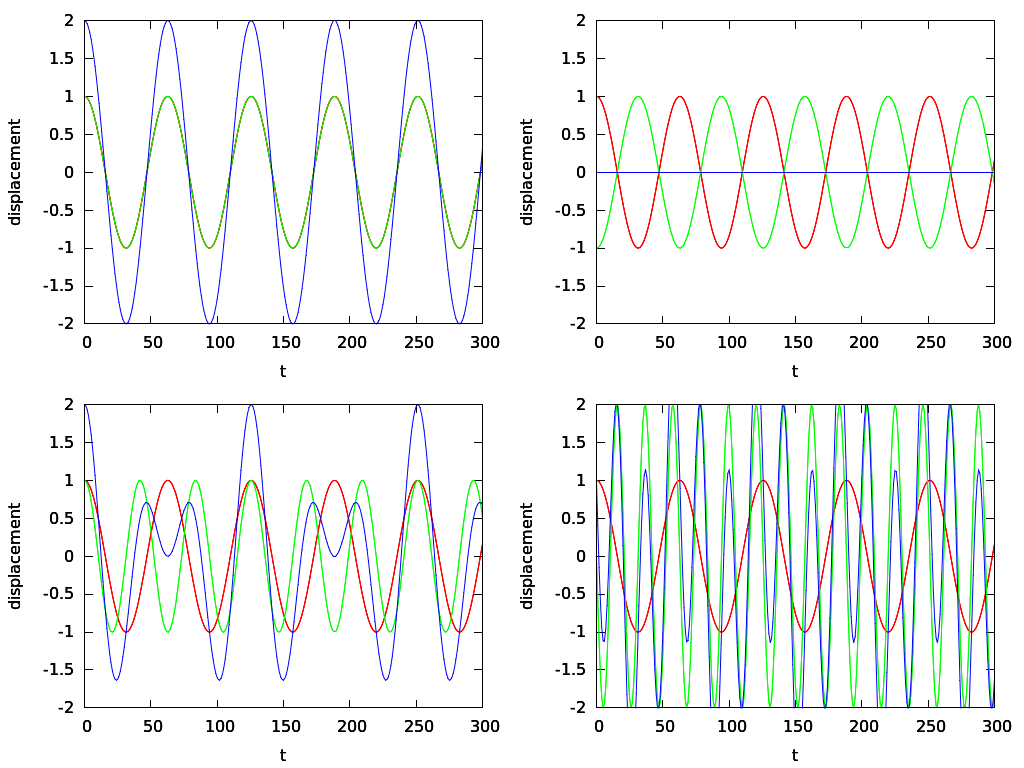
\includegraphics[width=\textwidth]{../result/simulation1.png}
\caption{两个简谐振动的合成.这四幅图(左上,右上,左下,右下)分别对应参数表\ref{tab:8},\ref{tab:9},\ref{tab:10},\ref{tab:11}.}
\end{figure}

\section{光的多缝衍射}
\subsection{基本原理}
均匀光源的夫琅禾费多缝衍射,在屏上的光强分布为
$$I = I_0(\frac{sin^2u}{u^2})(\frac{sin^2Nv}{sin^2v})$$
$$u = \frac{\pi}{\lambda}a sin\theta,v = \frac{\pi}{\lambda}d sin\theta$$
其中a是狭缝宽度,d是光栅常数,$\theta$是衍射角,$\lambda$是入射光波长,$N$是狭缝有效数目.

由物理规律和各量定义,各参数之间满足以下限制条件:
\begin{enumerate}
\item $d>a>\lambda$
\item d与a同数量级,a与$\lambda$差两个数量级
\item $u\neq 0, sinv\neq 0$
\end{enumerate}

\subsection{程序流程}
程序中每隔1个单位时间计算一次位移,为使得比较连续的曲线,应使得周期$T>>1$.

由于$T = \frac{2\pi}{\omega}$,故要求$w_1 \leqslant 0.1,\ w_2 \leqslant 0.1$.其他参数影响不大.

\begin{algorithm}[H]
\KwIn{$a,d,\lambda,I_0,N,file$}
\KwOut{a table of $\theta,I$ stored in $file$}
\For{$\theta =0;\theta<0.1;\theta+=0.0001$}{
	$u \gets \frac{\pi}{\lambda}a sin\theta$\;
	$v \gets \frac{\pi}{\lambda}d sin\theta$\;
	$tmp1 \gets \frac{sinu}{u}$\;
	\If{$tmp1$ is NaN}{$tmp1 \gets 1$\;}
	\If{$tmp1$ is Inf}{break\;}
	$tmp2 \gets \frac{sinNv}{v}$\;
	\If{$tmp2$ is NaN}{$tmp2 \gets N$\;}
	\If{$tmp2$ is Inf}{break\;}
	$I \gets I_0(tmp1^2)(tmp2^2)$\;
	print $\theta,I$ to $file$\;
}
 \caption{光的多缝衍射}
\end{algorithm}
在C/C++中,当除法分母为0.0时,计算结果是NaN(Not A Number).如果不判断的话,$\theta=0$时的计算结果就是错误的.在上面的算法中,我人为的将值赋为极限值.

\subsection{模拟及结果}
\subsubsection{模拟的参数设置}
\begin{table}[H]
\begin{minipage}[b]{0.3\linewidth}\centering
\begin{tabular}{cc}
\hline
$a(mm): 0.05$ &$d(mm): 0.1$\\
$\lambda(nm): 590$ &$I_0: 1$\\
$N: 1$ &\\
\hline
\end{tabular}
\caption{模拟1参数}\label{tab:5}
\end{minipage}
\hspace{0.5cm}
\begin{minipage}[b]{0.3\linewidth}\centering
\begin{tabular}{cc}
\hline
$a(mm): 0.05$ &$d(mm): 0.1$\\
$\lambda(nm): 590$ &$I_0: 1$\\
$N: 2$ &\\
\hline
\end{tabular}
\caption{模拟2参数}\label{tab:6}
\end{minipage}
\hspace{0.5cm}
\begin{minipage}[b]{0.3\linewidth}\centering
\begin{tabular}{cc}
\hline
$a(mm): 0.05$ &$d(mm): 0.1$\\
$\lambda(nm): 590$ &$I_0: 1$\\
$N: 5$ &\\
\hline
\end{tabular}
\caption{模拟3参数}\label{tab:7}
\end{minipage}
\end{table}

\subsubsection{模拟的图形结果}
\begin{figure}[H]
\centering
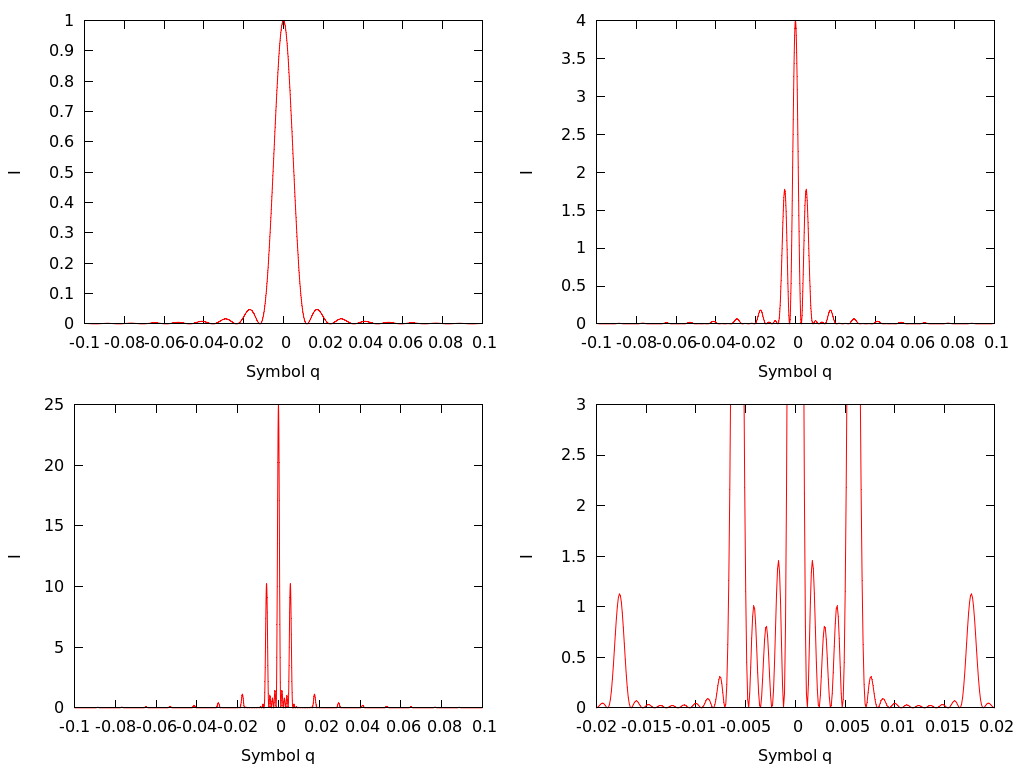
\includegraphics[width=\textwidth]{../result/simulation2.png}
\caption{$\alpha$粒子的散射模拟结果.前三幅图(左上,右上,左下)对应参数表 \ref{tab:5},\ref{tab:6},\ref{tab:7}.最后一幅图是参数表\ref{tab:7}的图形经放大形成的.}
\end{figure}


\section{$\alpha$粒子的散射}
\subsection{基本原理}
原子核的电荷为Ze,位置固定在坐标($x_0,y_0$),其质量远大于$\alpha$粒子.$\alpha$粒子电荷2e,其位置为(x,y).

当已知$\alpha$粒子初始坐标和速度,可以通过库仑力计算公式求得加速度:
$$F_x=2Ze^2(x-x_0)/R^3,\ F_y=2Ze^2(y-y_0)/R^3$$
$$a_x=\frac{2Ze^2}{m}\frac{x-x_0}{R^3},\ a_y=\frac{2Ze^2}{m}\frac{y-y_0}{R^3}$$

在微小的时间内,近似为匀加速运动:
$$v_x(t+dt)=v_x(t)+a_xdt,\ v_y(t+dt)=v_y(t)+a_ydt$$

在微小的时间内,近似为匀速运动:
$$x(t+dt)=x(t)+v_x(t+dt)dt,\ y(t+dt)=y(t)+v_y(t+dt)dt$$

由此即可得到$\alpha$粒子运动轨迹

\subsection{程序流程}
为便于计算和用户输入,仿照课本令$k=2Ze^2/m$

\begin{algorithm}[H]
\KwIn{$k(2Ze^2/m),x_0,y_0,x,y,vx,vy,file$}
\KwOut{a table of $x,y$ stored in $file$}
\For{$ t =0;t<5;t+=0.05$}{
	$R^3 = ((x-x_0)^2+(y-y_0)^2)^{3/2}$\;
	$a_x \gets k\frac{x-x_0}{R^3}$\;
	$a_y \gets k\frac{y-y_0}{R^3}$\;
	$v_x \gets v+0.05a_x$\;
	$v_y \gets v+0.05a_y$\;
	$x \gets x+0.05v_x$\;
	$y \gets y+0.05v_y$\;
	print $x,y$ to $file$\;
}
 \caption{光的多缝衍射}
\end{algorithm}
\subsection{模拟及结果}
\subsubsection{模拟的参数设置}
\begin{table}[H]
\begin{minipage}[b]{0.2\linewidth}\centering
\begin{tabular}{cc}
\hline
$k: 0.75$ &\\
$x_0: 0$ &$y_0: 0$\\
$x: -4$ &$y: 0$\\
$vx: 1$&$vy: 0.5$\\
\hline
\end{tabular}

\caption{模拟1参数}\label{tab:1}
\end{minipage}
\hspace{0.5cm}
\begin{minipage}[b]{0.2\linewidth}\centering
\begin{tabular}{cc}
\hline
$k: 0.75$ &\\
$x_0: 0$ &$y_0: 0$\\
$x: -4$ &$y: 0$\\
$vx: 1$&$vy: 0.1$\\
\hline
\end{tabular}

\caption{模拟2参数}\label{tab:2}
\end{minipage}
\hspace{0.5cm}
\begin{minipage}[b]{0.2\linewidth}\centering
\begin{tabular}{cc}
\hline
$k: 0.75$ &\\
$x_0: 0$ &$y_0: 0$\\
$x: -4$ &$y: 0$\\
$vx: 1$&$vy: 0.01$\\
\hline
\end{tabular}

\caption{模拟3参数}\label{tab:3}
\end{minipage}
\hspace{0.5cm}
\begin{minipage}[b]{0.2\linewidth}\centering
\begin{tabular}{cc}
\hline
$k: 0.75$ &\\
$x_0: 0$ &$y_0: 0$\\
$x: -4$ &$y: 0$\\
$vx: 2$&$vy: 1$\\
\hline
\end{tabular}\\

\caption{模拟4参数}\label{tab:4}
\end{minipage}
\end{table}

\subsubsection{模拟的图形结果}
\begin{figure}[H]
\centering
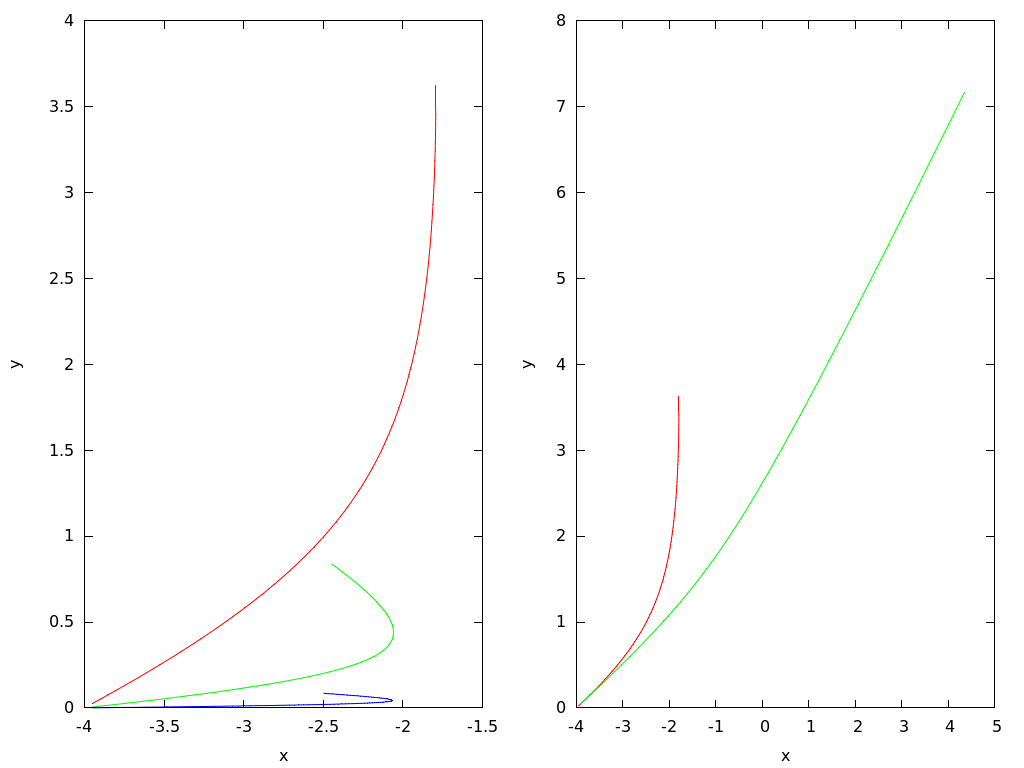
\includegraphics[width=0.7\textwidth]{../result/simulation3.png}
\caption{$\alpha$粒子的散射模拟结果.左图三条曲线红绿蓝对应参数表 \ref{tab:1},\ref{tab:2},\ref{tab:3}.右图两条曲线红绿对应参数表 \ref{tab:1},\ref{tab:4}.}
\end{figure}









\end{document}